\documentclass[12pt]{article}
\usepackage{lipsum}
\usepackage{listings}
\usepackage[margin=1in,left=1.5in,includefoot]{geometry}
\usepackage{graphicx}%Allows you to import images
\usepackage{float}% Allow for control of float position.
\usepackage{type1cm}%Allows you to control fonts size


\linespread{1}\selectfont %linespread

%Header and Footer Stuff
\usepackage{fancyhdr}
\pagestyle{fancy}
\fancyfoot{}
\fancyfoot[R]{ \thepage\ }
\fancyhead{}
\renewcommand{\footrulewidth}{1pt}
\renewcommand{\headrulewidth}{1pt}
%



\begin{document}

\begin{titlepage}
	\begin{center}
	\line(1,0){300}\\
	[0.25in]
	\huge{\bfseries Basic on MVC model \\ Personal Information and Java Online Test Website}\\
	[2mm]
	\line(1,0){200}\\
	[1.5cm]
	\textsc{\LARGE Lan Zhou Jiao Tong University}\\
	[0.75cm]
	\textsc{\LARGE Engineer Faculty}\\
	[0.75cm]
	\textsc{\LARGE Dissertation}\\
	[3cm]	
	\end{center}
	\begin{flushright}
	\textsc{\normalsize Hao Bang\\
	\#201110417\\
		August 10,2015\\}
	\end{flushright}
	
	
	
	
	
\end{titlepage}
%Front matter stuff
\pagenumbering{roman}

\section * {Summary}
\addcontentsline{toc}{section}{\numberline{}Summary}
   This is my dissertation for graduating from Lan Zhou Jiao Tong University in 2015, which I wrote in Japan while guided by Dr. Ken Higuchi. Actually I really want to create my own website by myself, so before I graduate from Lan Zhou Jiang Tong University, I decided to create it here as my graduation paper. I decided to use mysql as the database and Tomcat + Eclipse as my operated tools.
   
   For the user: this website, which can be used in daily life and practise Java knowledge, uses "Auto Running " to process. This system was developed based on the MVC model. It has 5 functions including "Login",''Register","Personal Information","Java Online test","Contact". And each of them has their own JSP, Servlet and JavaBean.  It also connects to the mysql database.  People can use this website to test what score they can get and which part of the Java need to practise . From section two - six introduce the user's functions .  
   
   For the manager: It also has website pages to manage its user information like email address or question and choices. Section Seven is for the manager(Super User) who can change the question for the users.
   
   But for this website, it still has a lot of weaknesses and insufficiencies. Because the main point for making this website is to familiarise users with Java language and mysql database. So it still needs a lot of time and patience. As for the next step, I want to study SSH frameworks to re-organize this website.  
   
   
     
     
\cleardoublepage


%\section * {Acknowledgements}
%\addcontentsline{toc}{section}{\numberline{}Acknowledgements}
%Thanks to my teacher and sdasdasdasd.
%\cleardoublepage
%This is table of contents stuff
\tableofcontents
\thispagestyle{empty}
\cleardoublepage 

%List of figures,list of tables
\listoffigures
\addcontentsline{toc}{section}{\numberline{}List of Figures}
\cleardoublepage


%This is main body stuff
\pagenumbering{arabic}
\setcounter{page}{1}



%Chapter One : Introduce
\section{Introduction}\label{sec:intro}
	In this website the main purpose is to create an automatically running operation system. In this system, people can do a test in  different kinds of questions and different number of questions. When we start to learn new things not only in Java, we need to practise and remember a lot of basic skills. As the meaning for this Website system, which is help user practise and remember their knowledge, is absolutely important in our daily life . So with Higuchi sensei 's advise, I decided to make this online test website.
	
	From the beginning of this paper, I have studied a lot of coding languages, like HTML, CSS, JavaScript , mysql and Java Web. Although it was just for the really basic knowledge, they can still achieve the functions of this system. In HTML, I have learnt how to create a basic website and how to post the information with JavaScript validation. About the CSS, it is really necessary for website creation, because it can decorate the website and make it more fancy and more clear. As for the Java Web, which is amazing that people create this stuff to create website, it can help people to create an interactive website, not just a static page in the browser, and make the website more variable.  Mysql, which is totally free and useful for the database beginner like me, can help me get familiar with the database. For the sake of future learning, Mysql is a basic and useful tool.
	
	From Higuchi sensei' s advise and teaching, I have revised this system a lot of times, like how to make its function more powerful or how to make the database table more clear. 
Last for three months, I think, I created this website system and wrote this paper.  The detail of this website system will be illustrated from  section two to section seven.
	
	At last I want to say, thanks to Lan Zhou Jiao Tong University who gave this opportunity to me. I am really honoured to have stayed in Japan for a year as an international student and to be Higuchi sensei's student in Fukui University.

\newpage

%Chapter Two :Objective
\section{Objective}
	For this website page, I want to create a project which I achieved by myself.  I create my own project which will help me improve my architecture design in programming. For the sake of improving my programming skills and becoming familiar with Java and database knowledge and basic skills. I have chosen Java and Mysql as my basic tools. For creating a website system, HTML and CSS are necessary. All of them were new technologies for me three months ago.  But now, I have created a new system by myself. It is really impressive and encouraging for me to create my own system.
	
	The first reason to create this system is that I can familiarise myself with the Java Programming language and the database knowledge in order to create more bigger Web System.
 	The second reason I created this website is because of my guide teacher's advise that it will help me to learn more knowledge not only in Java.
	Although this web system still has a lot of problems and weaknesses, it also have a long way to study and practise. But I have got the confidence, I think I can do that ! 








\cleardoublepage




%Chapter Three : System
\section{System}









\subsection{Overview}
	In the website system, I have used Java programming language  (JSP Servlet and JavaBean )and mysql as database to build online test system.  HTML, CSS and JavaScript have also used in this web system.  Two kinds of account has been demonstrated . 
	
	For the user: there are five functions has been displayed in here included " Login " , " Register " , " Personal Information " , " Online test " and " Contact us " . The user can use this website to test their knowledge in Java and manage their personal information . If the user have some opinions or advices to test this website , he can use the 'contact us' page to write the comment to the manager.   Here is the navigation page in this website after the user has logged in .
	\begin{figure}[H]
	\centering
	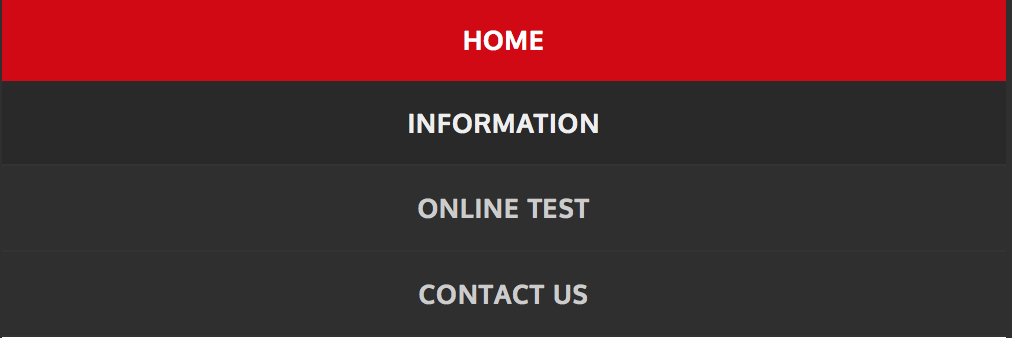
\includegraphics[width=13cm]{images/Navigation.jpg}
	\caption[Navigation page]{Navigation Page}
	\label{fig:Navigation Page}
\end{figure}
	For the manager : the manager can edit the test question and check the information (password not included )from the user. Also the user 's comment when users use the "Contact us " function will be seem by the manager.
	
	
	
	
	The whole system is based on the Model-view-controller(MVC) a software architectural pattern for implementing user interfaces.  It will make the logical more clearly. And the user can see the view via the JSP page and logic controller through the Servlet . As for the model I have use the JavaBean to store the user's information.
\begin{figure}[H]
	\centering
	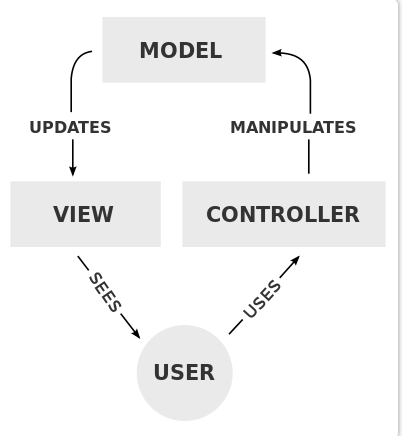
\includegraphics[height=1.5in]{images/MVC.jpg}

	\caption[MVC page]{MVC Page}
	\label{fig:MVC Page}
\end{figure}

\cleardoublepage

\subsection{\ Login Function}
Login function is really basic function in the website design . Nearly 90 percent of the websites will use the login and register page . So in here I have used the JSP(JavaServlet Page)  and Servlet and JavaBean to create this login page. Here is the login page picture:
	\begin{figure}[H]
	\centering
		%\includegraphics[height=2in]{../../Desktop/123123.jpg}
		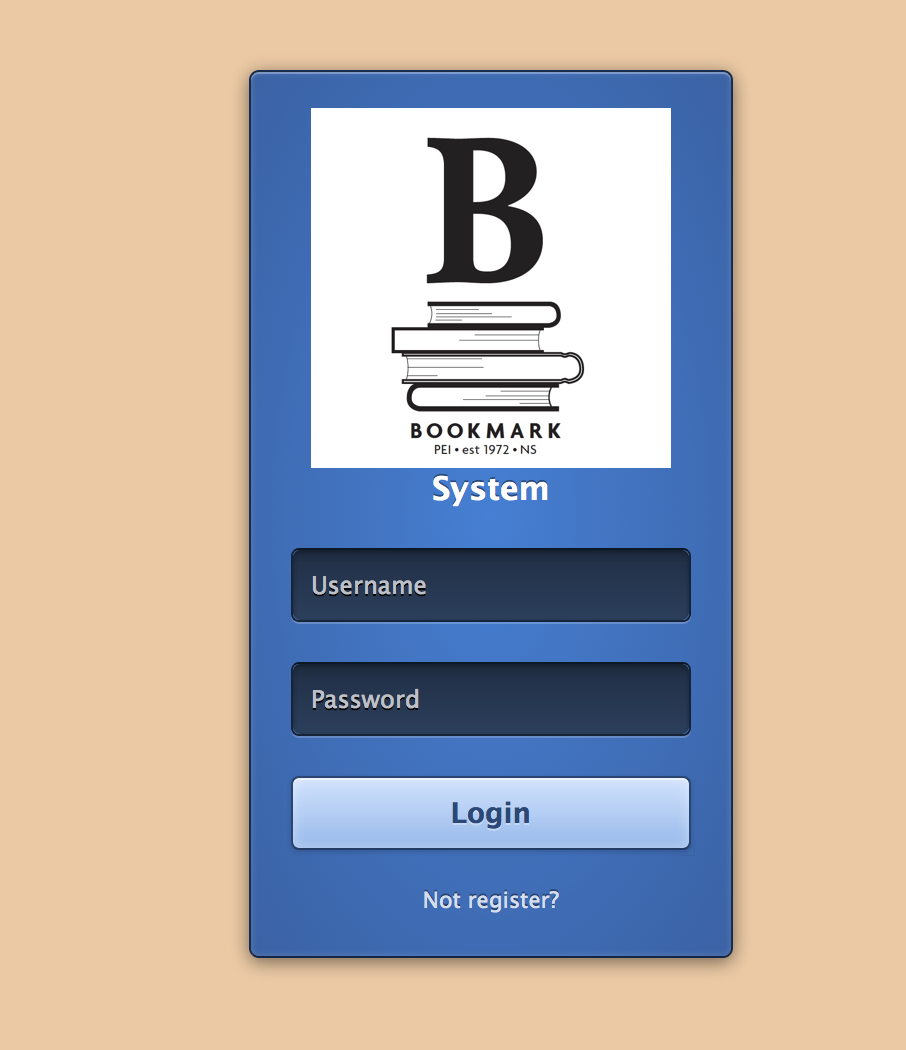
\includegraphics[height=6in]{images/loginPage.jpg} 
	\caption[Login page]{Login Page}
	\label{fig:loginPage}
\end{figure}
	In this page people can login to the main Page of this website.  People input with username and password. It will connect to the Mysql database to check it is correct or not . As for the database table ,  I will show in the next chapter .  
	\subsubsection{Login Page: Jsp}
\begin{figure}[H]
	\centering

		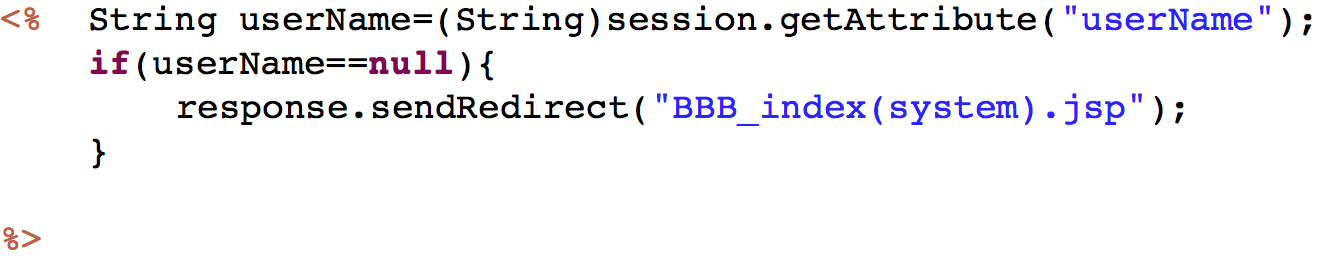
\includegraphics[width=15cm]{images/Check Login Code.jpg}
	\caption[Check Login Code]{Login Check Code}
	\label{fig:onlinetest}
\end{figure}
	
	In this code  in  here has demonstrated  that if user didn't login that the page will redirect to the login page. This part of code has put nearly in every JSP page in this system.
	In this login JSP page I also used JavaScript to check the information has input or not. This is the example in here :
%Here we insert into figure
\begin{figure}[H]
	\centering
		%\includegraphics[height=2in]{../../Desktop/123123.jpg}
		
		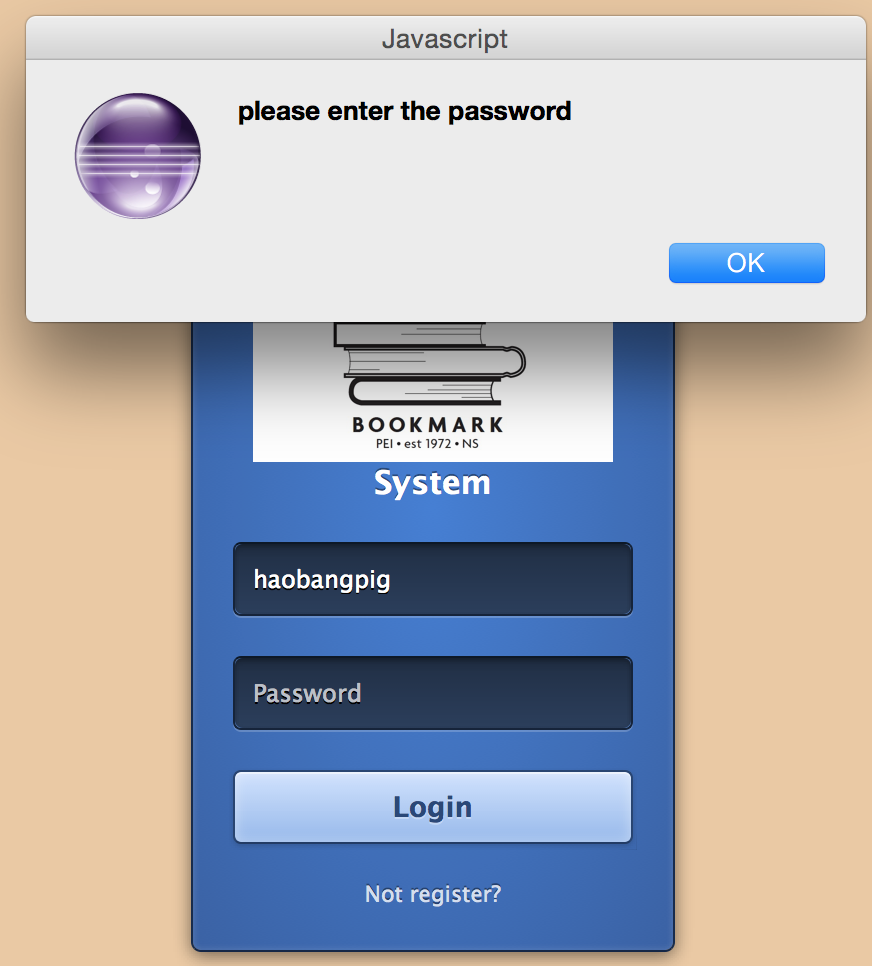
\includegraphics[height=4in]{images/JavaScriptCheckImage.jpg}

	\caption[JavaScript Check Image]{JavaScript Check}
	\label{fig:JavaScript Login}
\end{figure}
	
%Figure \ref{fig:onlinetest} shows the database.\cite{ref:two}
	
\cleardoublepage	

\subsubsection{Login Page: Servlet}
Servlet : When I first known this concept,  I was really confused . I didn't know what is it and how to code it . Even with the most basic program like "Hello World " in servlet. But in here I used the Servlet to get the data from the "login.jsp" and connect to the mysql database and check  it whether correct or not.  
	If the username and the password can find in the mysql database table , than the page will redirect to the main page . If the username or password is incorrect , than  it will redirect to the error page and ask the user try again. 
	 Here is the error page in here :
	\begin{figure}[H]
	\centering
		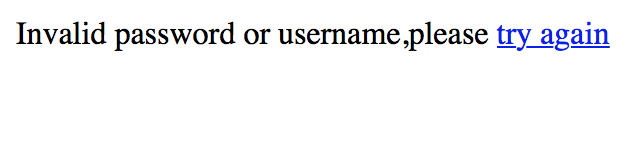
\includegraphics[width=15cm]{images/loginError.jpg}
		\caption[Login Error]{Login Error Page}
	\label{fig:loginErrorPage}
\end{figure}


\subsubsection{SuperUser}
In the register.java(Servlet) which I have edited a new function : if the Username equal "haobangpig" and the Password equal "haobang123"  then the page will redirect to the SuperEdit.jsp ( It can be seem in the Chapter 7)  where the manager can  edit the user's information and the questions.  But in here , I didn't use CSS to create this Page. Just use the form in the HTML to fulfill these part of function . Like delete and edit the user's information or the questions. (If you want to know more ,please check the Chapter 7: SuperUser). And here I will shown how it works to redirect to the SuperUser.jsp:
\begin{figure}[H]
	\centering
		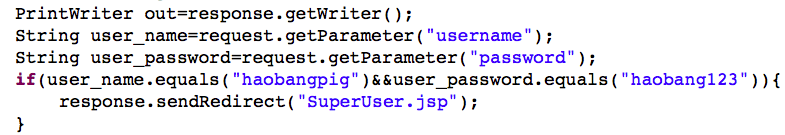
\includegraphics[width=15cm]{images/SuperUserRedirect.jpg}

		\caption[SuperUserRedirect]{SuperUserRedirect}
	\label{fig:SuperUserRedirect}
\end{figure}


\newpage
%Chapter Three.3
			
\subsection{Register Function}
The Register Function is one of the most import and basic function in a website system. In order to better comprehend and edit this part of function , I have searched the Internet that JSP pages shouldn't do any logical operation . Just demonstrate or post the message and information to the control layer. Here is the figure about Register page:
\begin{figure}[H]
	\centering
		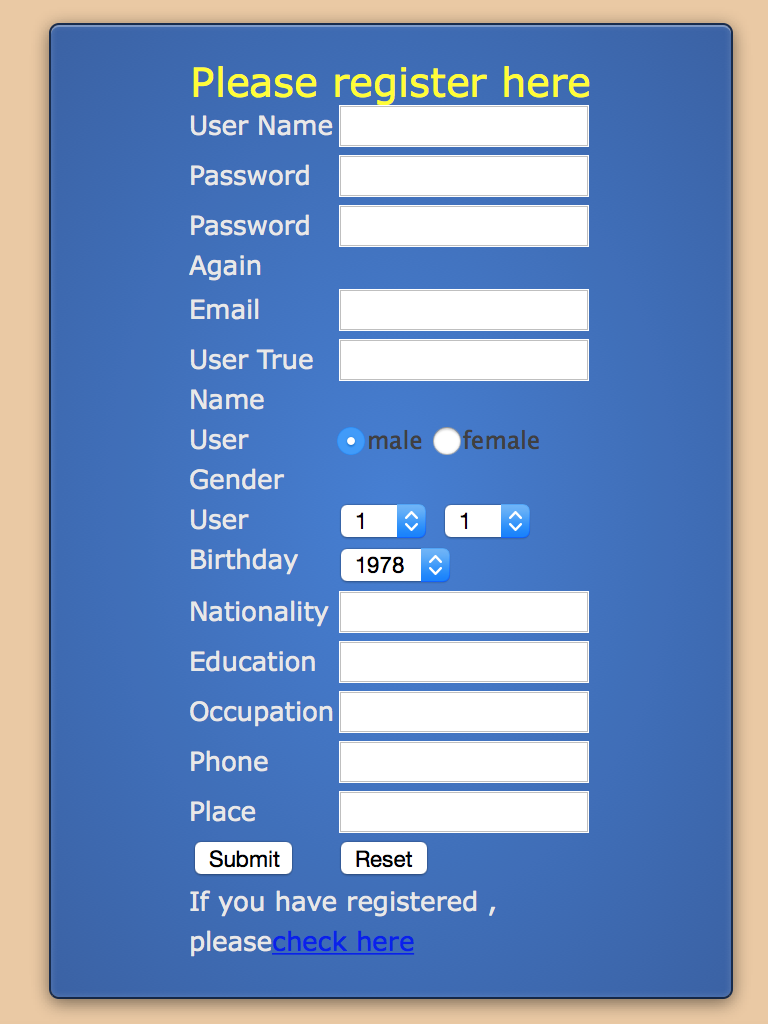
\includegraphics[height=6in]{images/RegisterPage.jpg}

		\caption[Register Page]{Register Page}
	\label{fig:Register Page}
\end{figure}
	 The three components will be described in the next three section which included their main sources or output pages.
\cleardoublepage
	


\subsubsection{Register : Mysql User table}
In this section , I will describe the most important table which has used in this web system included the information of the users will be display in here:
\begin{figure}[H]
	\centering
		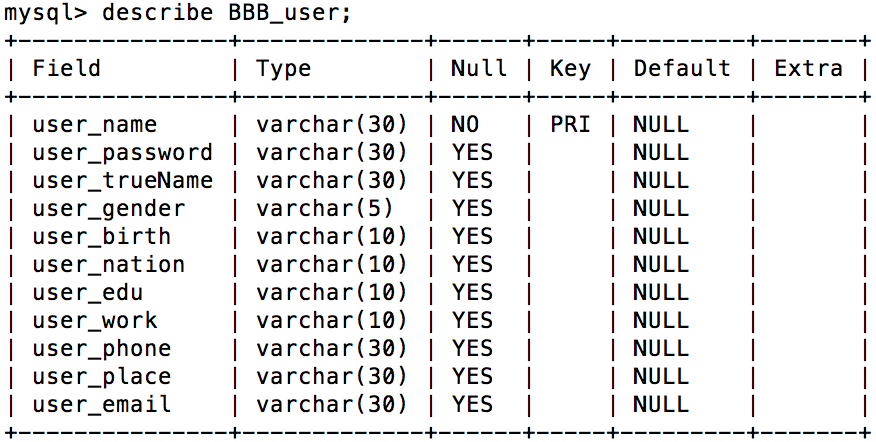
\includegraphics[height=3in]{images/MysqlUserTable.jpg}
		\caption[MysqlUserTable]{MysqlUserTable}
	\label{fig:MysqlUserTable}
\end{figure}
	From the figure in here, the user table has included the username , password , email address and others important information. About the username  in here , I have set the username as the primary key in this table which can help us inspect the username without repeating.
	Although the table in here is lack of the security and the rigorousness, but it can still satisfy for the fundamental web system. As the table in here we can get a clear logic that user input their username and password or others information though the JSP page and send to the Servlet which can  retrieve these information  and store to the mysql database.  Thus , we can interpret this logic as  in the follow sections.
\cleardoublepage









\subsubsection{Register Page: Jsp}
So in this Register JSP , in order to more concise and easy to edit the user page in here . I have created  a  form in here which contain plenty of  input where the user can put its own information there. In other way , I also have used JavaScript in here to check the information  which is really important to the user like username and password and email  address, which can be combined with HTML to check the information. This is the main source in JavaScript:
\begin{figure}[H]
	\centering
		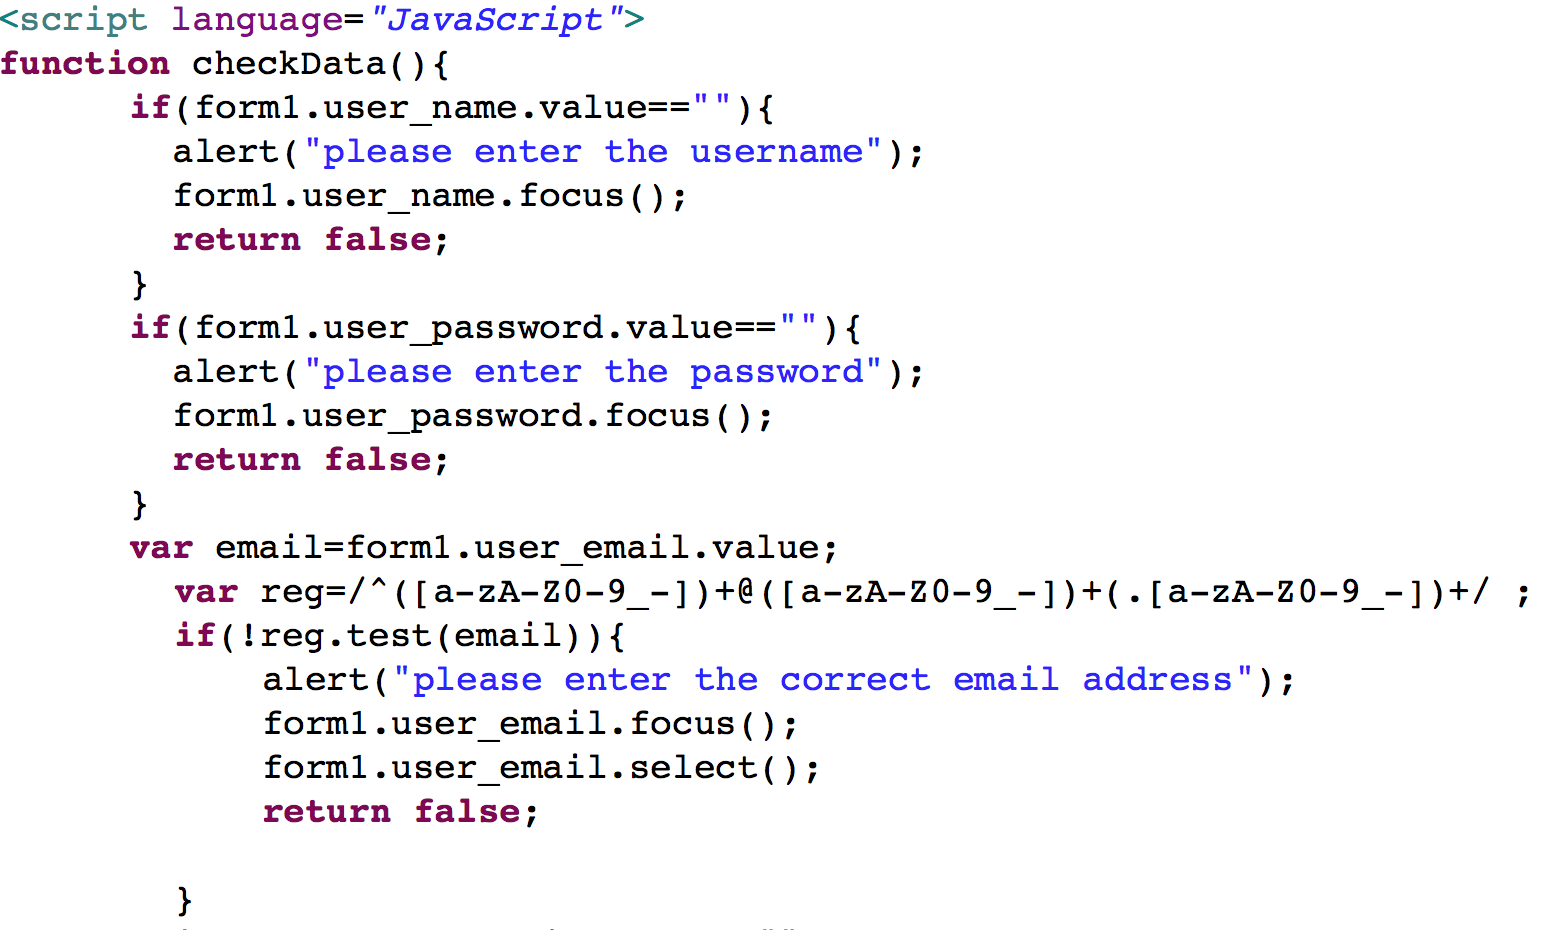
\includegraphics[width=15cm]{images/RegistJavaScript.jpg}


		\caption[Register JavaScript Code]{Register JavaScript Code}
	\label{fig:Register JavaScript Code}
\end{figure}
The primary purpose is to check the user whether he is input or not .  And  Regular Expression is used in here to check if the user input is available in the email address. If you enter the incorrect email address format , than it will display like this : 
\begin{figure}[H]
	\centering
		
		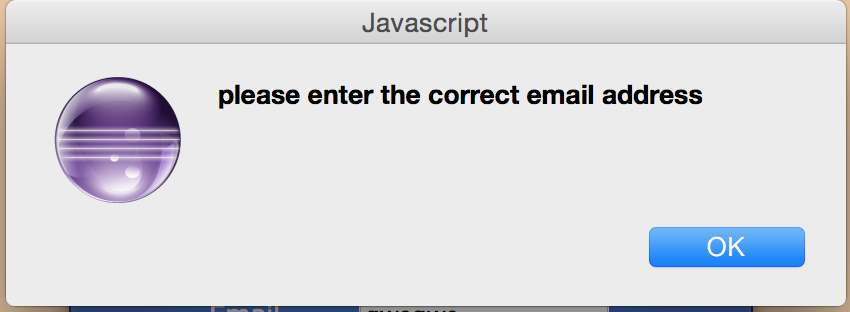
\includegraphics[width=10cm]{images/RegisterEmailIncorrect.jpg}


		\caption[RegisterEmailIncorrect]{RegisterEmailIncorrect}
	\label{fig:RegisterEmailIncorrect}
\end{figure}



\newpage
\subsubsection{Register Page: Servlet}



In this section, I will provide the basic functions which are retrieve the data from the Register JSP and store them to the mysql database. This is  the main code in this function :
\begin{figure}[H]
	\centering	
	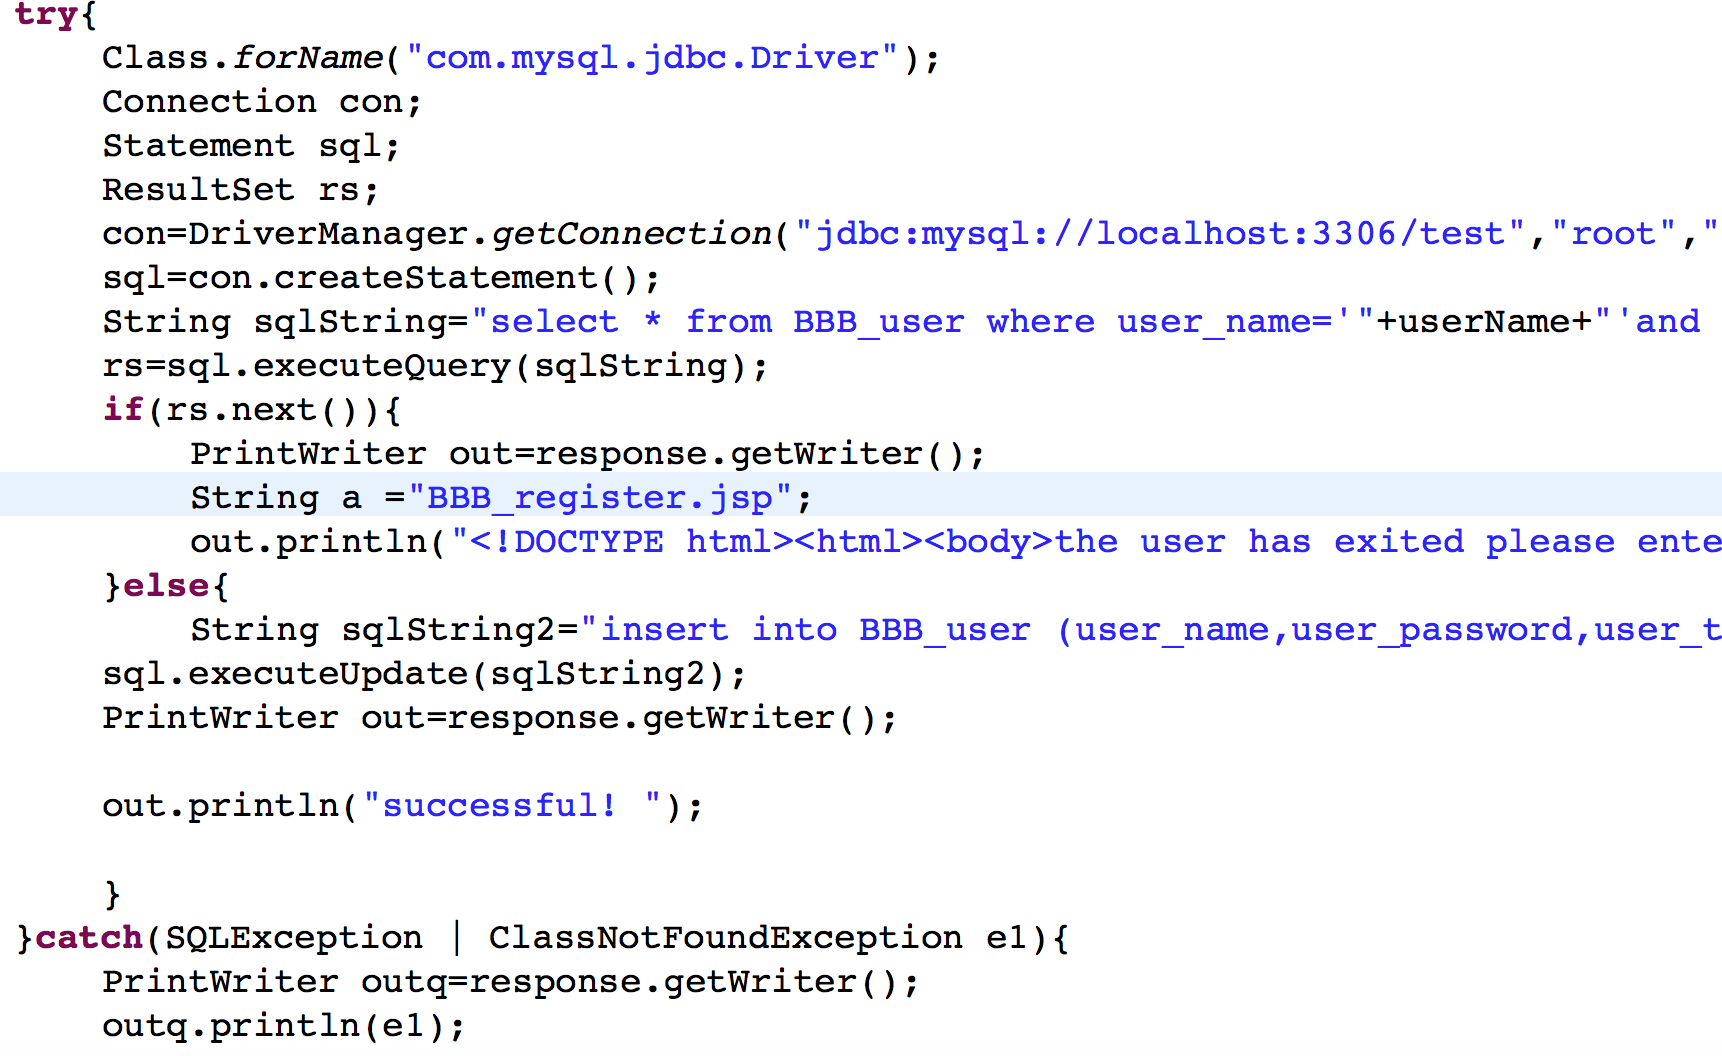
\includegraphics[width=15cm]{images/RegisterServletMainCode.jpg}
	\caption[RegisterServletMainCode]{RegisterServletMainCode}
	\label{fig:RegisterServletMainCode}
\end{figure}

As we can see in this figure illustrated in here has demonstrate the logic of this part . If we input the username which has existed in our mysql(database)'s user table , than we can get the error page like this:
\begin{figure}[H]
	\centering	
	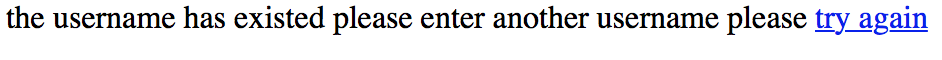
\includegraphics[width=15cm]{images/RegisterSameUsernameError.jpg}

	\caption[RegisterSameUsernameError]{RegisterSameUsernameError}
	\label{fig:RegisterSameUsernameError}
\end{figure}

	If we click the "try again " URL, we will be redirected to the Register Page.

\newpage

%Chapter three.4

\subsection{Personal Information}
One of the key and basic function of a personal information manage website system is that the personal information edit page. In order to better security , I have created a JSP page which is special for changing password. With the time limited, I just created the basic  page in here without any decorating .There are three branch illustrated in here :
\begin{figure}[H]
	\centering	
	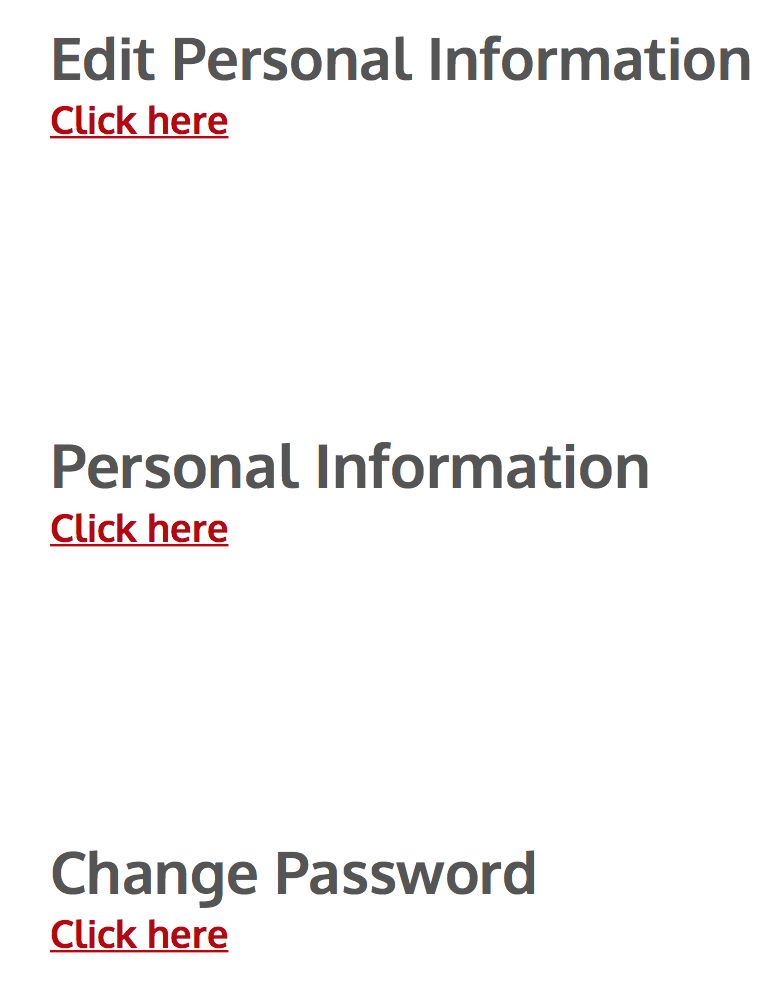
\includegraphics[height=3in]{images/EditPersonalInformation.jpg}

	
	\caption[EditPersonalInformation]{EditPersonalInformation}
	\label{fig:EditPersonalInformation}
\end{figure}


This is part of the main source which use HTML basic character to redirect to another page. In each of the page has its own function in here.
\begin{figure}[H]
	\centering	

	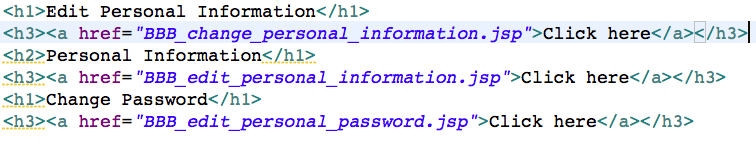
\includegraphics[width=15cm]{images/EditPersonalInformationMainSource.jpg}

	\caption[EditPersonalInformationMainSource]{EditPersonalInformationMainSource}
	\label{fig:EditPersonalInformationMainSource}
\end{figure}

\newpage



\subsection{Personal Information : Personal Information}
The user who can see his personal information, but the password which can't be seem in here .  The information which was input by the user when he register in this web system is stored into the user database . And in here this JSP page retrieve the information and show them. For the sake of security , the password can be edited in the other page.  

For my original design idea in here , Creating a  friends contacts in here , and people can add friends with each other and share their opinion about the test and the test questions. But the function need more information , but in the future I think it may be done if I use the SSH framework .  And the next step is to create more function in here .

\begin{figure}[H]
	\centering	
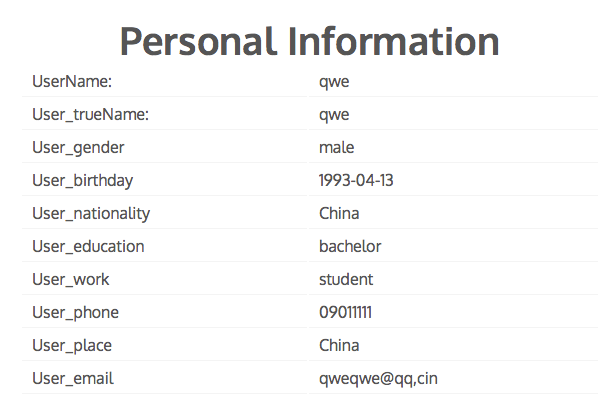
\includegraphics[width=15cm]{images/PersonalInformation.jpg}
	\caption[PersonalInformation]{PersonalInformation}
	\label{fig:PersonalInformation}
\end{figure}
\newpage




\cleardoublepage

\subsubsection{Personal Information : Edit Information}
As well as registering in the registerPage.jsp , we can edit our information here, but the username can't be changed. 

\begin{figure}[H]
	\centering	
	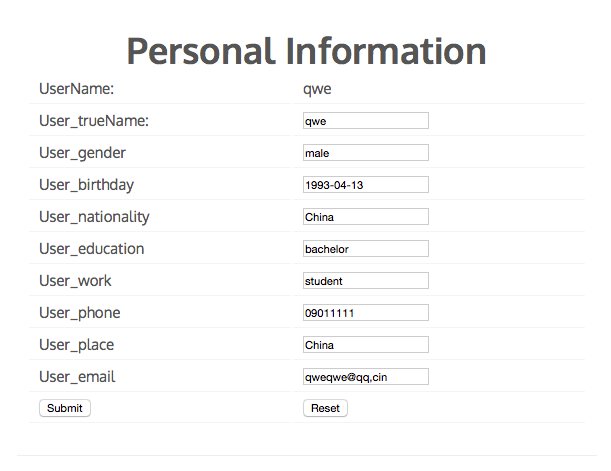
\includegraphics[height=3in]{images/EditInformation.jpg}
	\caption[EditInformation]{EditInformation}
	\label{fig:EditInformation}
\end{figure}

The logic retrieved the data from the database and then shown in this page is obviously in here. Using HTML5 characteristic set input 's values equals the database sources. Here is the main souce in here.
\begin{figure}[H]
	\centering	
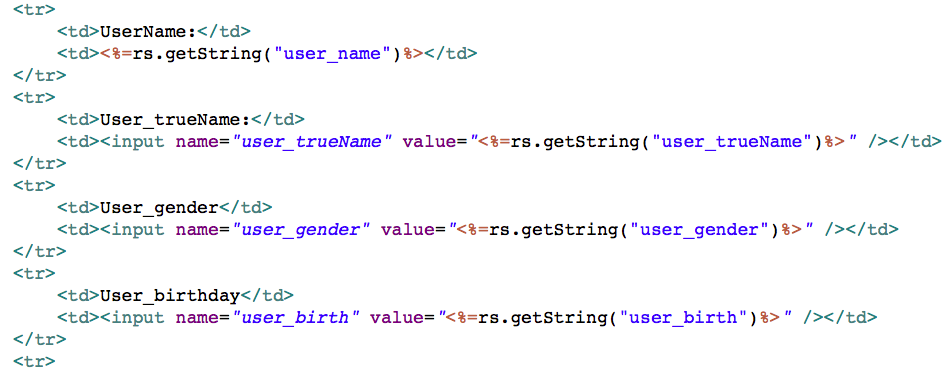
\includegraphics[width=15cm]{images/EditInformationMainSource.jpg}

	\caption[EditInformationMainSource]{EditInformationMainSource}
	\label{fig:EditInformationMainSource}
\end{figure}
\cleardoublepage



\subsubsection{Personal Information : Change Password}
Password which is the most important and difficult problem  for web system developer . I have search for a lot of data about how to protect the password and how to improve our user account security. For example like filter in JSP , I think I need more time and patience to study in  JAVA , not only in Java Web , but also in Java basic knowledge like implements, interface or extend. But in here , I just wanna show you about this function changing the password.Here is the user interface:
\begin{figure}[H]
	\centering	
	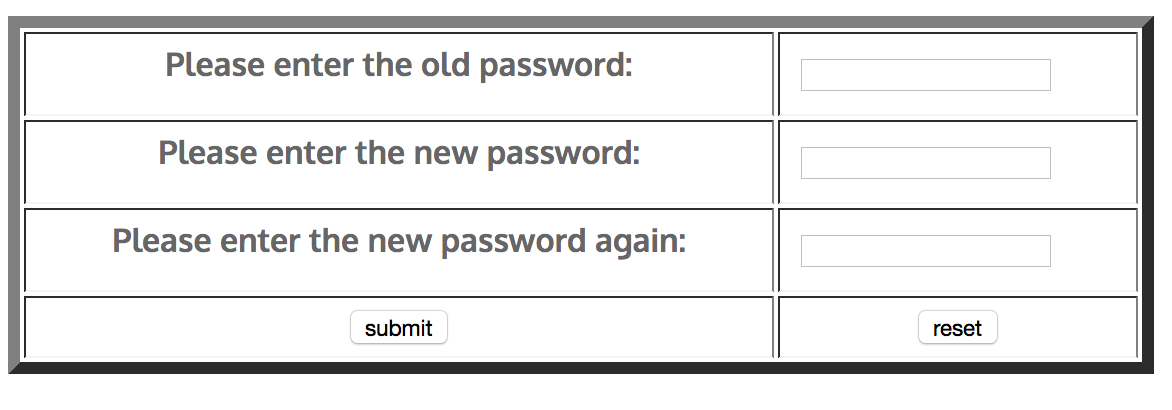
\includegraphics[width=15cm]{images/UserChangePasseword.jpg}

	\caption[UserChangePasseword]{UserChangePasseword}
	\label{fig:UserChangePasseword}
\end{figure}
The logic in changing user password is obviously. The user will input the old password first , and the two times of the new password which will be checked by the JavaScript , and then the page will redirect to the next page which can detect the the old the password is correct or not . If the password is incorrect , this series of actions will be rejected . Only if the old password is correct , then the password will be changed . Here is  the main code of changing password:
\begin{figure}[H]
	\centering	
	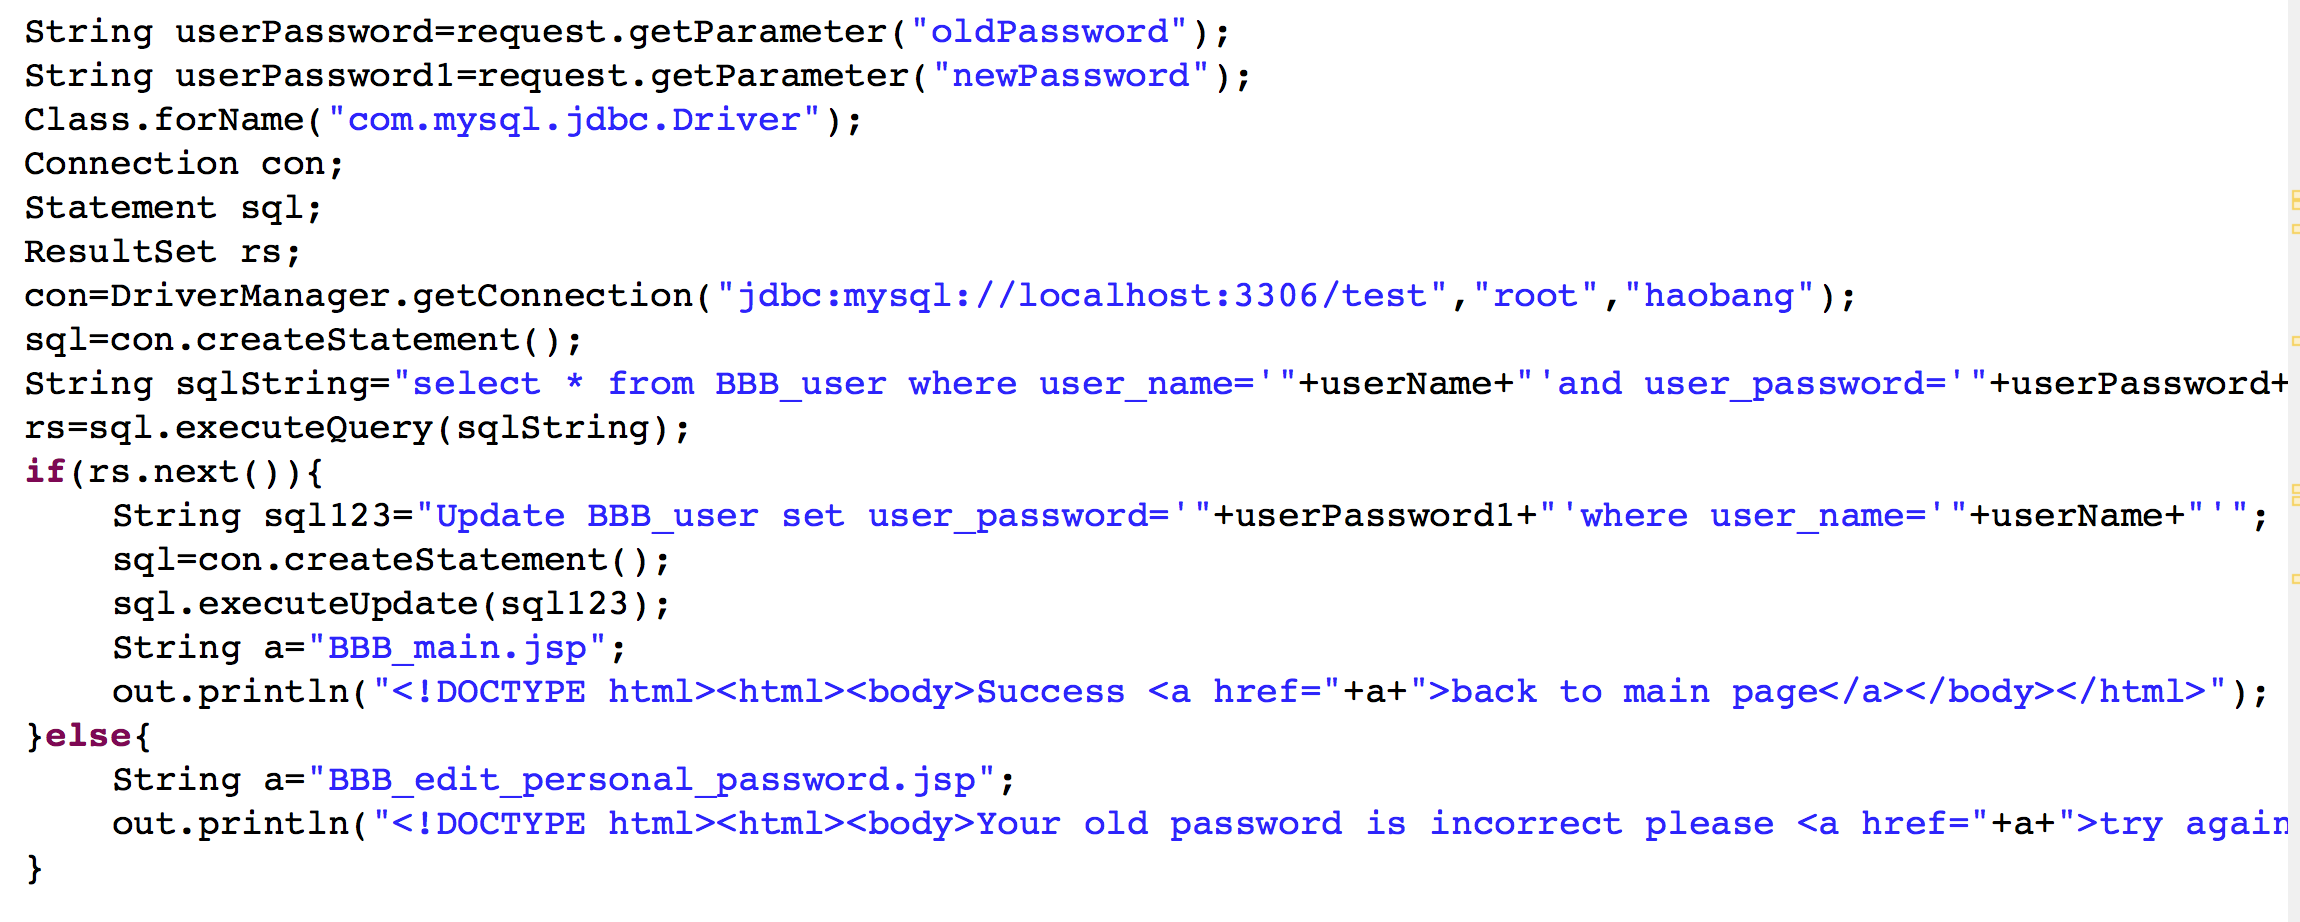
\includegraphics[width=15cm]{images/UserChangePasswordMainCode.jpg}

	
	\caption[UserChangePasswordMainCode]{UserChangePasswordMainCode}
	\label{fig:UserChangePasswordMainCode}
\end{figure}
 	It has shown that the JSP will connect to the mysql database first and execute the sql command (select  all from user where name=XXX, and password = XXX)  which means the page retrieve the user 's information and check the old password which has input from the previous page is correct or not. If it isn't correct, it will output like this :
\begin{figure}[H]
	\centering	
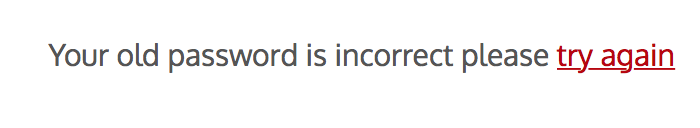
\includegraphics[width=15cm]{images/UserChangePasswordFail.jpg}

	
	\caption[UserChangePasswordFail]{UserChangePasswordFail}
	\label{UserChangePasswordFail}
\end{figure}
As the two times input in the previous page will be detected by the JavaScript which I have used for user registering. This is the main code about it :

\begin{figure}[H]
	\centering	
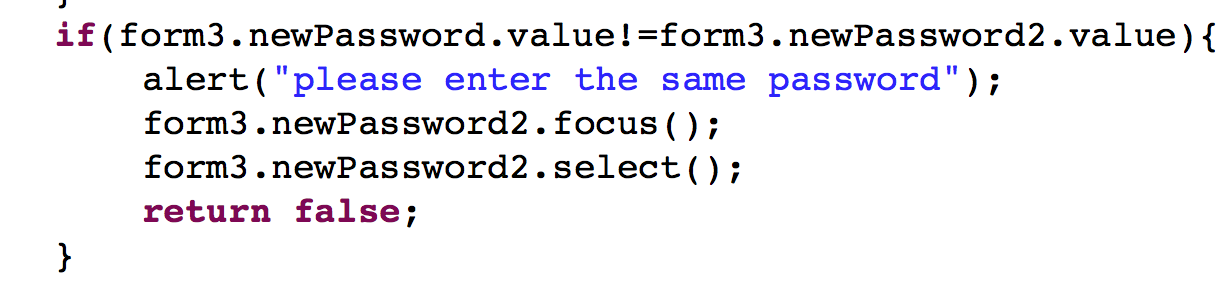
\includegraphics[width=15cm]{images/UserChangePasswordTwoTimesCheck.jpg}

	
	\caption[UserChangePasswordTwoTimesCheck]{UserChangePasswordTwoTimesCheck}
	\label{UserChangePasswordTwoTimesCheck}
\end{figure}
For these sections , although it has a lot of weakness and insufficient, but after studying the basic part of JSP and servlet . And for the next section , it will display the main part about this dissertation which has included the auto-running idea and help us learn more not only in Java.
\cleardoublepage
%Chapter three.5		
\subsection{Java Online Test}
The Online Test, which can help us learn more about the knowledge and help us review about the knowledge. In this system , I just create the Java Online test. But the others questions test will be the same . The super user can edit the questions and add some questions into the database, This is user interface in Online Test :
\begin{figure}[H]
	\centering	

	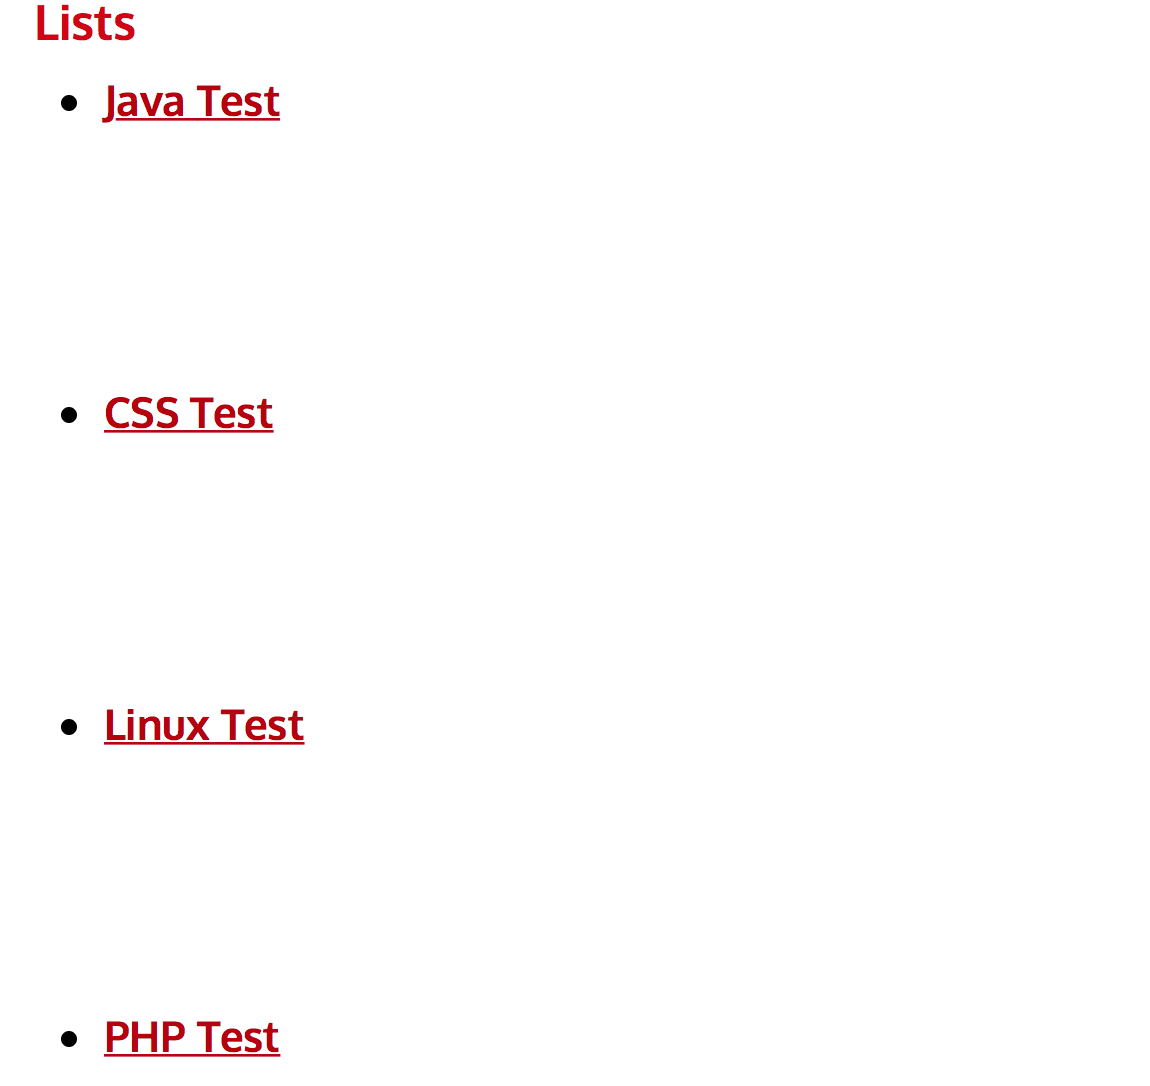
\includegraphics[height=4in]{images/OnlineTestUserInterface.jpg}

	\caption[OnlineTestUserInterface]{OnlineTestUserInterface}
	\label{OnlineTestUserInterface}
\end{figure}



	In this user interface , if you click the button except the 'Java Test' , it will redirect to a blank page . Because I didn't create the others page in here . 
	
	If you click the 'Java Test' , redirecting to the Java page and starting the test immediately.  There are three steps in one level and I have created two level in here. Each of the level have three steps: ' Arrays ', ' Files Input and Output' and ' Introduction' . In level one , I set each step with three questions . if you can't get above 20 points(total is 30) , you will get to the circle with the different questions but the same catalogue. 
	Logic is like this :
	\begin{figure}[H]
	\centering	
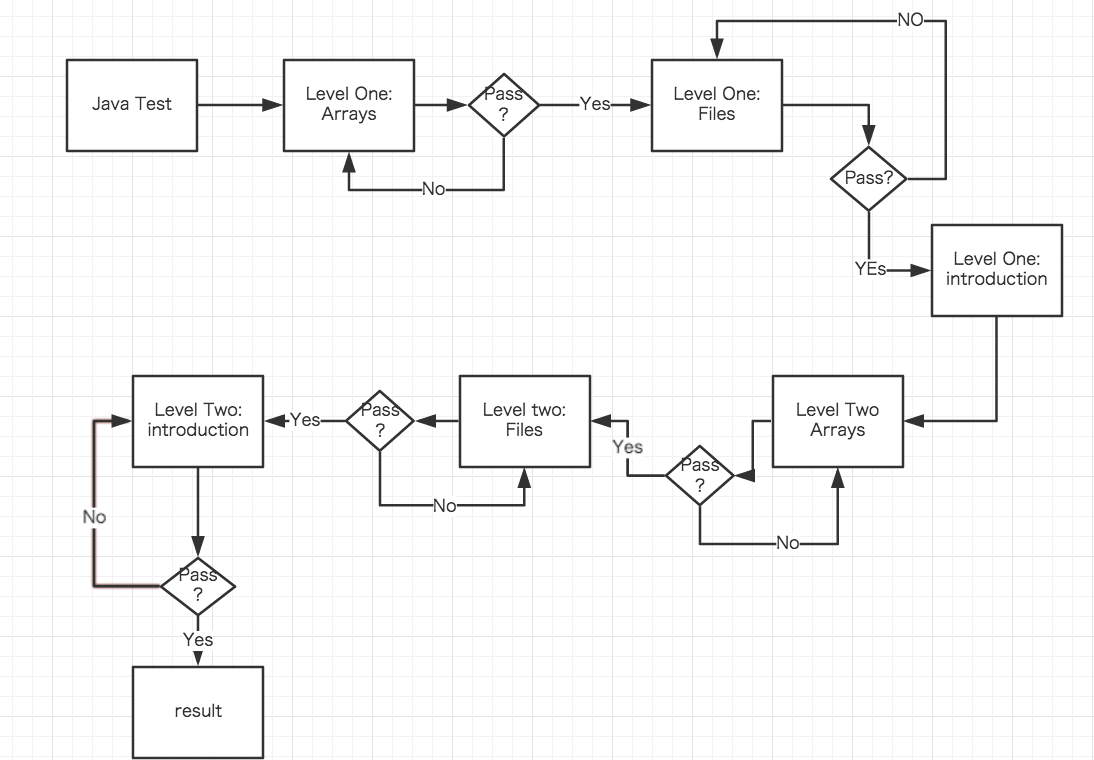
\includegraphics[width=16cm]{images/JavaTestLogic.jpg}



	\caption[JavaTestLogic]{JavaTestLogic}
	\label{JavaTestLogic}
\end{figure}
	
	
	
	After you finished the level one in here , you can enter the level two of Java Test. But in level two , the number of the question will depend on the situation which will be calculated by the computer . The information will be accumulated by the JSP via the user who use this system. The number of the questions in here will be detected by the computer . If in the level one and the same catalogue the number of correct answer is above the incorrect answer number, the system will set three as its number of question in the same catalogue on level two. Conversely, the system will set six as its number of the question.
	
	
	
	
\cleardoublepage
\subsubsection{Java Online Test : Mysql database table}
	About the database table , I have create six question tables and one accumulation table in this system . I will shown you two of them .

	\begin{figure}[H]
	\centering	
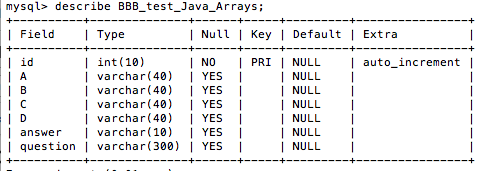
\includegraphics[width=15cm]{images/JavaTestQuestionList.jpg}
	\caption[JavaTestQuestionList]{JavaTestQuestionList}
	\label{JavaTestQuestionList}
\end{figure}
	In this table ,  we can see the questions and their choices are included. Set the question id as primary key and automatically increment is helpful for us to see the results in the next table.
		\begin{figure}[H]
	\centering	
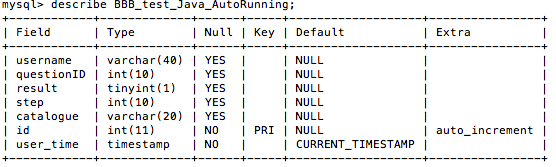
\includegraphics[width=15cm]{images/JavaTestRecord.jpg}

	\caption[JavaTestRecord]{JavaTestRecord}
	\label{JavaTestRecord}
\end{figure}
	 Username, questionID, result, step, catalogue and time has been given. In this record, people can see their record and help them to realise  their questions and in which part of the Java they need to improve. Also , in these two tables in here can help superuser to edit and manager questions and this web system. 
\newpage


\subsubsection{Java Online Test: Circle}
	The logic flow chart has been shown in this section , and about the circle ,  if the user can't get above 20 in level one or less than 30 in six number of questions in level two , it will redirect into the circle page . There are two circles in one step, as long as you can get score above 20 in level one or 30 in level two , it will go to the next step.  
\begin{figure}[H]
	\centering	

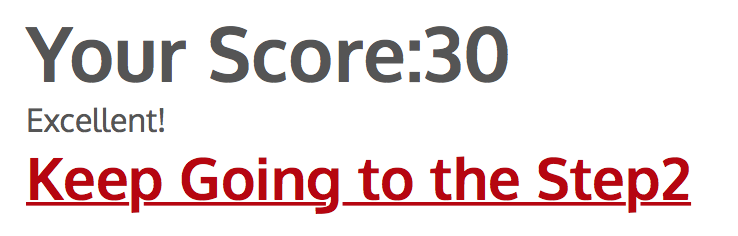
\includegraphics[width=11cm]{images/JavaTestCircle.jpg}

	\caption[JavaTestCircle]{JavaTestCircle}
	\label{JavaTestCircle}
\end{figure}
	And each of the circle in here will be shown the different questions in the question list . For example , I didn't pass the Level One Arrays from question 1-3 , then it will give 4-6 to the user in the circle. 
	
\subsubsection{Java Online Test: Auto Running}
Auto Running system in web system , it will automatically calculate the result which has been stored into the database when the user start to participate the Java test. Here is the main code about the auto running :
\begin{figure}[H]
	\centering	

	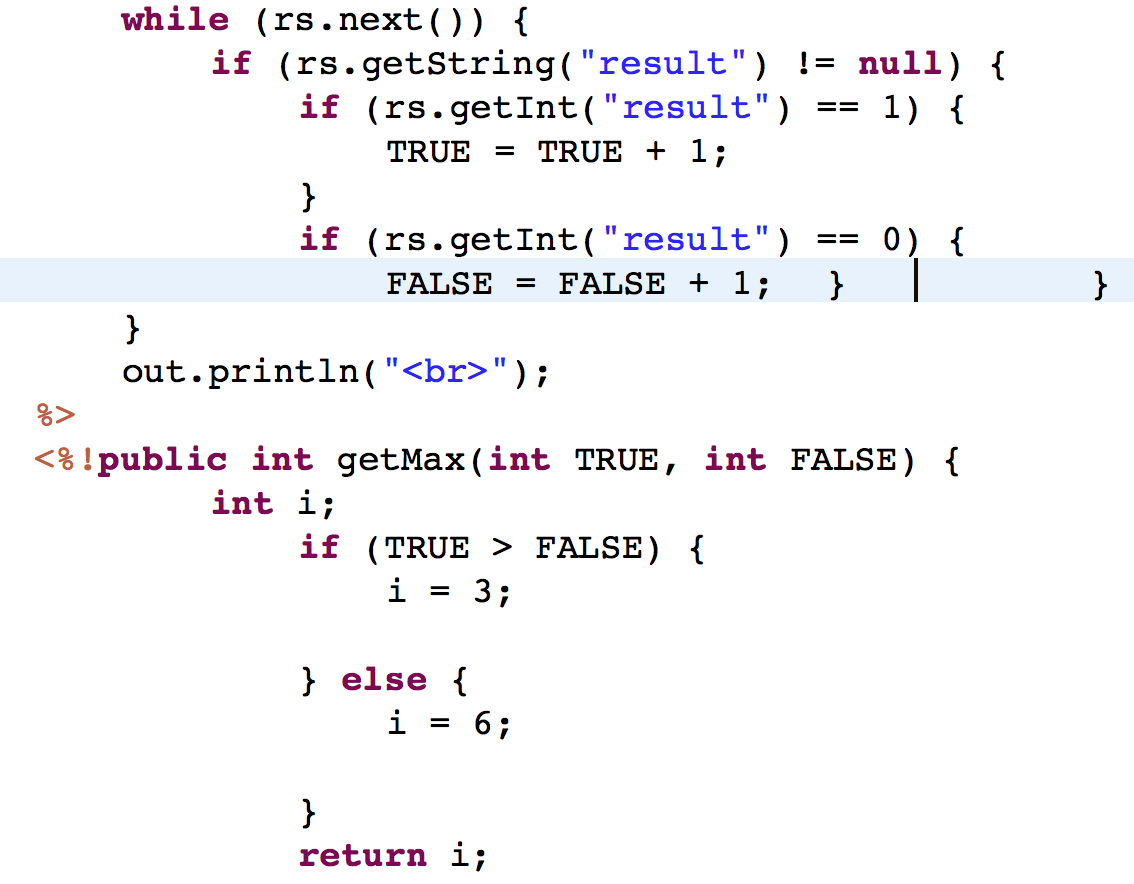
\includegraphics[height=3in]{images/AutoRunningMainCode.jpg}

	\caption[AutoRunningMainCode]{AutoRunningMainCode}
	\label{AutoRunningMainCode}
\end{figure}




\subsubsection{Java Online Test: Result}
After participating the test in this website , The user can see their result which can help user review and concentrate on the weak point. It is basic on the user who have already done the test and the data have already stored into the database  which has been shown in the section 5.1.  And the result can display the user in which part of Java should be concentrate on and in which part should be review in Java  . Here is the result page :
\begin{figure}[H]
	\centering	
	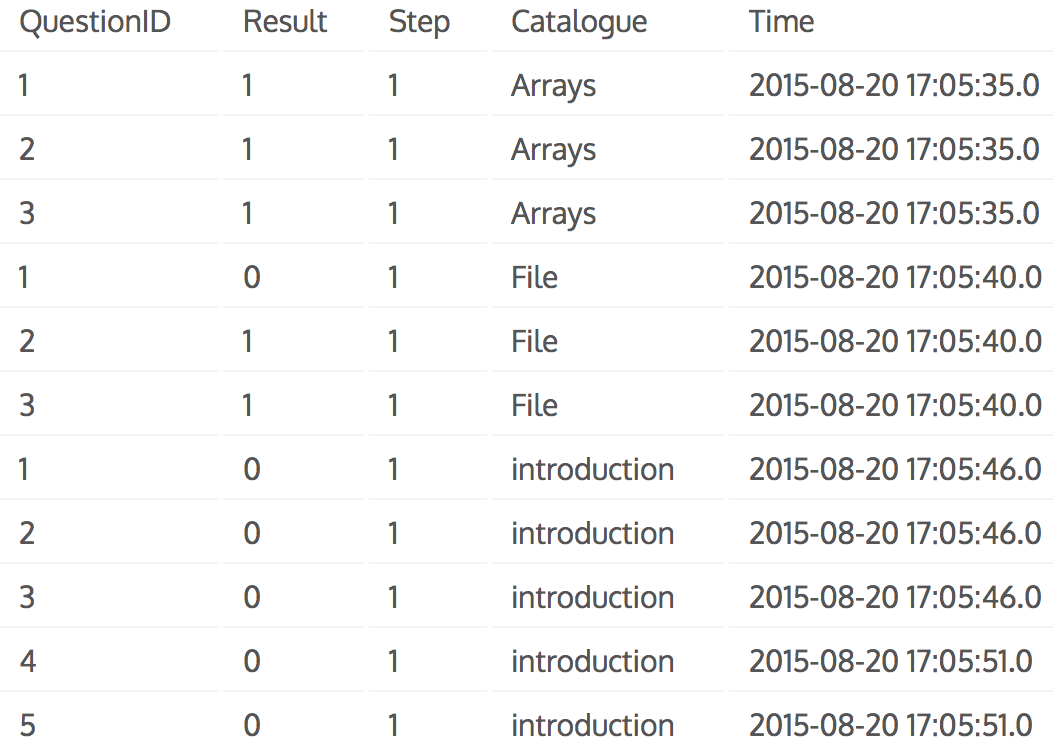
\includegraphics[width=15cm]{images/TestResult.jpg}


	\caption[TestResult]{TestResult}
	\label{TestResult}
\end{figure}

	In this page , the user can see The question ID , result, step, catalogue and time . In the result, 1 equal correct and 0 equal incorrect . As for the catalogue ,  it is really important for the user to see which part of knowledge need to review and study. About the time which can record the user  when participate the test is obviously for the user. 
\newpage

%Chapter three.6	
\subsection{Contact Us}
This is the really basic function in the website system, because the user can comment this system and give them advise to make this system better. So the website in here , I just create the name, email-address which can help us to contact him easily and comment. And the comment  will display for the superuser This is page in here :
\begin{figure}[H]
	\centering	
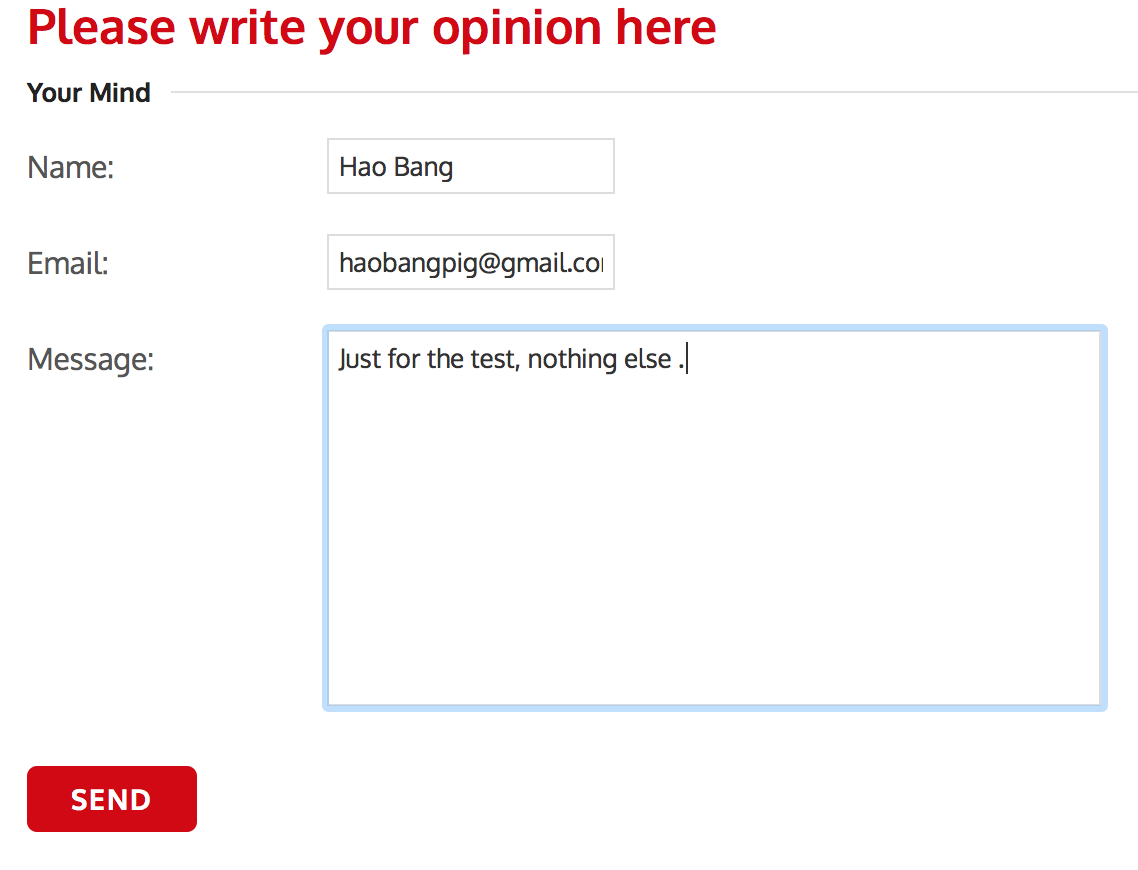
\includegraphics[width=15cm]{images/ContactPage.jpg}
	\caption[ContactPage]{ContactPage}
	\label{ContactPage}
\end{figure}

After clicking  the send button in this page, it will redirect into the next page and display like this :

\begin{figure}[H]
\centering	

\includegraphics[width=10cm]{images/ContactSuccess.jpg}
\caption[ContactSuccess]{ContactSuccess}
\label{ContactSuccess}
\end{figure}
\newpage


%Chapter three.7
\subsection{Super User}
Super User , who is as a manager in this web system,  can edit the questions and see the user information .  Without decorating , the superUser page may a little be ugly , but the function in here has be achieved. The super User functions are editing the questions and check the information for the user . So here is the page about the superUser :
\begin{figure}[H]
\centering	
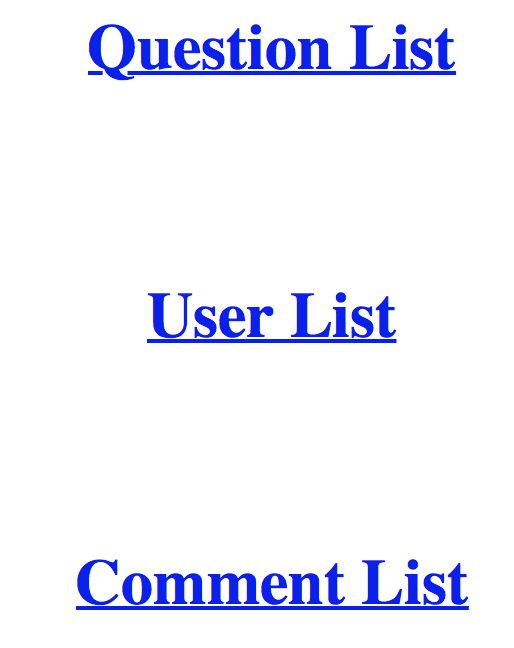
\includegraphics[height=2in]{images/SuperUserFunction.jpg}
\caption[SuperUserFunction]{SuperUserFunction}
\label{SuperUserFunction}
\end{figure}

In the question list , the super user can edit the question like create a new question or change the old question 's choice . 
\begin{figure}[H]
\centering	
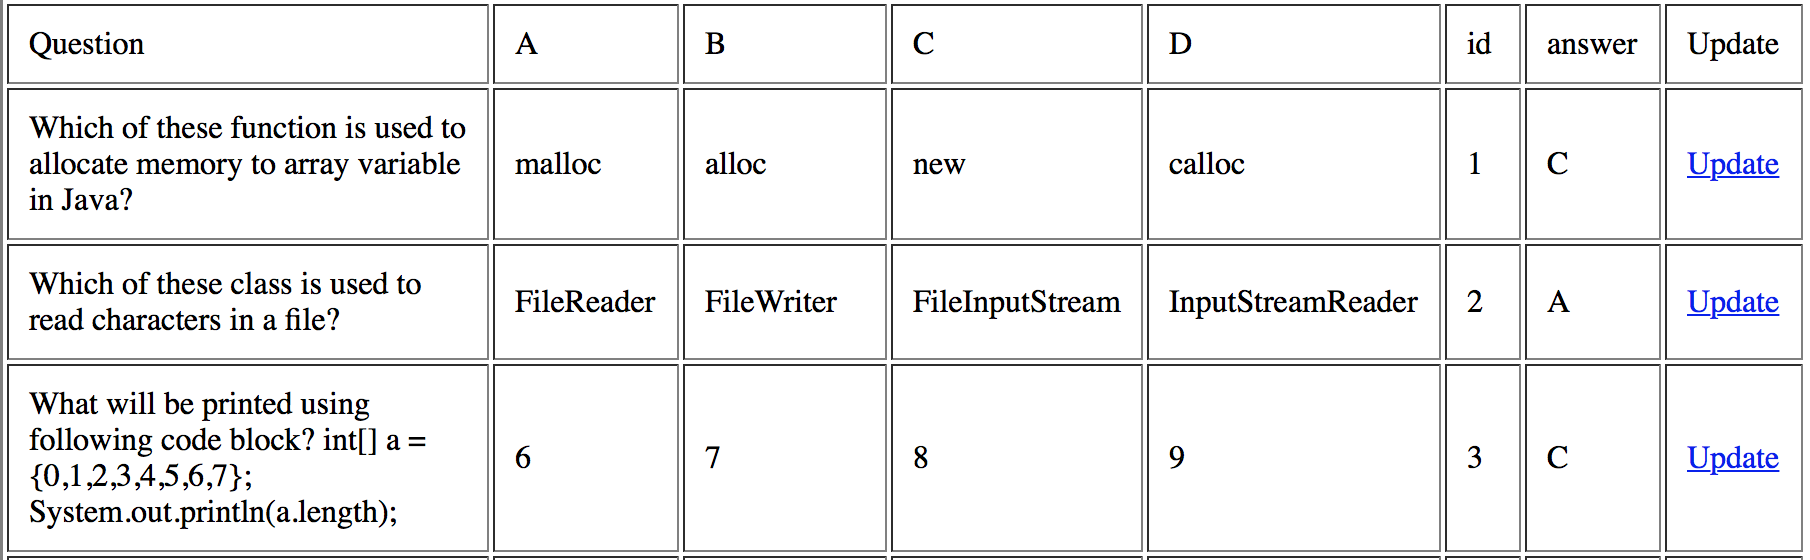
\includegraphics[width=15cm]{images/SuperUserEditQuestion.jpg}
\caption[SuperUserEditQuestion]{SuperUserEditQuestion}
\label{SuperUserEditQuestion}
\end{figure}
This is a page about the super user can change the question or choice. In the bottom of this page , there is a sentence call 'create a new question ' where super user can create a new question in the database. 

	As for the user list and the comment list , the super user click the URL and redirect into corresponding page and show the data from the database. I would like to show the comment database and page in here . The user list 's database have shown in the chapter 3 . 
\begin{figure}[H]
\centering	
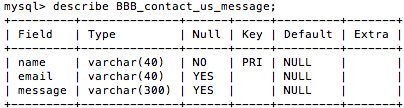
\includegraphics[]{images/SuperUserContactDatabase.jpg}

\caption[SuperUserContactDatabase]{SuperUserContactDatabase}
\label{SuperUserContactDatabase}
\end{figure}

This is the database structure . I have set the name as the primary key.  And the data have been stored into the mysql database in the command page . 
 \begin{figure}[H]
\centering	
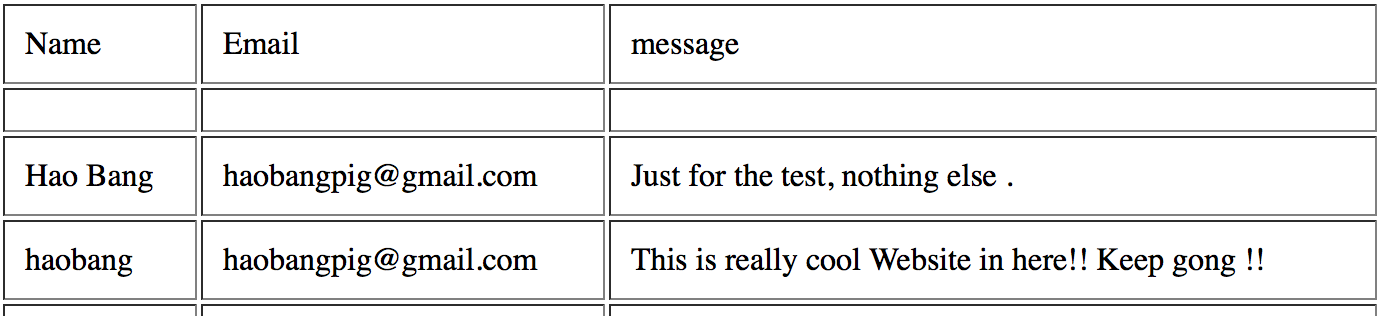
\includegraphics[width=15cm]{images/SuperUserContactPage.jpg}


\caption[SuperUserContactPage]{SuperUserContactPage}
\label{SuperUserContactPage}
\end{figure}


Super user can see the information from the users , and give them more choice in Test . Although, it is a kind of ugly page in here , because I didn't use any css or JQuery to decorate it . %I have to say it is really fun for creating my own website. It has still a lot of problems or weakness in this website , but I think it will be better as long as I amn't give up . 
\cleardoublepage



%Chapter Four : Conclusions and future work
\section{Conclusions and Future work}

	In creating this whole web system which I have introduced before has created "Auto-Running" Java Online test and personal information, I have learned a lot of knowledge and skills in Java Web development. 
	
	In the future study, I will use SSH framework in this Java Web System and I want to make the database table more efficient. I also want to learn about managing the data when the data has more than a million units and what kind of technologies or skills would be needed.
	
	 At last, I want to say thank Ken.Higuchi sensei as this paper 's guide teacher and Felix for helping me to review this paper.


\cleardoublepage


\addcontentsline{toc}{section}{\numberline{}Reference}
\bibliographystyle{IEEEtran}
\thispagestyle{empty}
\bibliography{/Users/banhao/Documents/dissertation/reference/reference.bib}






\end{document}